\documentclass[11pt]{report}

\usepackage{url}
\usepackage{graphicx}
\usepackage{xcolor}
\usepackage{mdframed}
\usepackage[framed,numbered]{mcode}
\usepackage[cc]{titlepic}

\title{paPAM \\ \Large User Manual for version 0.872}
\author{Developed by:\\ Sophie L. Nedelec, James Campbell, Andrew N. Radford,\\Stephen D. Simpson, Nathan D. Merchant}
\titlepic{\vspace{10cm} 
\includegraphics[scale=0.2,clip = true,trim = 0 0 0 0]{Uni_logo.png}}

\begin{document}

\maketitle

\tableofcontents

\chapter{Setting up paPAM} \label{SettingUppaPAM}

paPAM is written in MATLAB, therefore you need MATLAB to execute the program.  If you do not have a working version of MATLAB on your computer you can download MATLAB compiler runtime, a freely available program distributed by Mathworks for executing Matlab scripts.

\section{MATLAB}
paPAM was built and tested on MATLAB version \textbf{R2013a}.  While we've tried to make paPAM compatible with older versions of MATLAB, due to the different libraries of functions used across versions, some compatibility issues may arise when using versions other than R2013a.  If you cannot get paPAM working on your version of MATLAB, you can download and use MATLAB compiler runtime instead.

To run paPAM with a full version of MATLAB, all you need to do is open the folder \texttt{paPAM}, then run the file:\\\\ \texttt{PM\_Analysis\_GUI\_Windows.m}

\section{MATLAB Compiler Runtime}

MATLAB compiler runtime (MCR) is a free version of MATLAB available on the Mathworks website.  To install MCR, go to the Mathworks website and download the file corresponding with the version of MATLAB paPAM was compiled in:\\\\
\texttt{mathworks.com/products/compiler/mcr/}\\

As this version of paPAM was compiled in \textbf{R2013a (8.1) 32-bit} on windows, this is the version of MCR which you will have to download and install.  For Mac and Linux users, you'll have to download the MCR version \textbf{R2013a (8.1) 64-bit}

After MCR is installed, it will not be shown in your \texttt{All Programs} menu (or in your \texttt{Applications} folder for Mac users).  To run the MCR, all you have to do is double click the \texttt{paPAM.exe} file provided to you and MCR will automatically open the program.

\subsection{Using MCR on OSX and Linux}
Using MCR on UNIX computers (Mac and Linux operating systems) requires an extra step.  The steps are the same for both Linux and Mac operating systems.  To run a MCR file, you have to change some environment variables within the operating system.  A small script will be included with the \texttt{paPAM.app} file (\texttt{paPAM} on Linux) which will do this for you.  To run paPAM on Mac OSX, follow these steps:
\begin{enumerate}
\item Find the location of the MCR installation on your hard drive.  By default, MCR is installed in the folder: \\\\
\texttt{/Applications/MATLAB/MATLAB\_Compiler\_Runtime/v81}\\

Once you have located the MCR installation, keep it open in the finder.

\item Open the terminal (\texttt{Terminal.app}) and change your working directory to where ever you choose.  The working directory will be where all your temporary files are stored during the analysis.

Example: \texttt{cd \url{~}/Desktop}

\item Now open a new finder window and find the MCR paPAM files.  You should now have two finder windows open in addition to the terminal.\\\\

\begin{center}
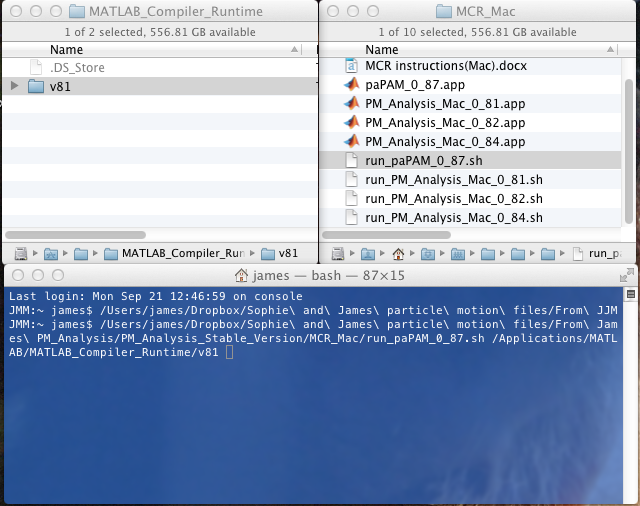
\includegraphics[width = \textwidth]{1.png}
\end{center}

\item Drag and drop the file \texttt{run\_paPAM.sh} into the terminal window, followed by the folder \texttt{v81}.  By dragging and dropping items into the terminal, you'll be automatically copying their locations to the terminal window.  Your terminal command should now look something like the image above.

\item Press \texttt{Enter}, and the terminal will execute the command and open paPAM in MCR.

\textbf{Note:} The file \texttt{paPAM.app} must be in the same folder as \texttt{run\_paPAM.sh} for this to work.
\end{enumerate}

\chapter{Using paPAM}

\section{Reciever Calibration files} \label{CalibrationFiles}

paPAM allows users to analyze vector and hydrophone data that has been recorded either simultaneously or separately. Receivers and recorders must both be calibrated.  Here we describe how to use manufacturer-provided receiver sensitivities for vector sensors and hydrophones in paPAM.  Vector sensors typically provide voltage as an output which then has to be converted into the relevant velocity or acceleration units.  Hydrophones also typically provide voltage as an output which then has to be converted into the relevant pressure units.  To convert voltage into useful acoustic metrics, we need to define the receiver sensitivity values for your specific device(s).  Receiver sensitivity values used by paPAM should be formatted in the following units:

\begin{enumerate}
	\item Pressure: $ \mathit{dB}\ (\ \mathit{re\ 1\ V/\mu Pa})$
	\item Velocity: $\mathit{dB} \ (\ \mathit{re\ 1\ V/\left(m/s\right)})$
\end{enumerate}

paPAM calibrates your data by transforming the raw voltage data into the frequency domain then applying the relevant calibration values to each frequency.  paPAM then converts the calibrated frequency domain data back into the time domain for analysis.

To be read by paPAM, the receiver sensitivity values should be arranged into an 8 column \texttt{.csv} file, where rows \texttt{[1 3 5 7]} hold the frequency ranges and rows \texttt{[2 4 6 8]} hold the respective receiver sensitivity values in dB units.

\begin{samepage}

 From the left to right, your values should be arranged in the \texttt{.csv} file by: \texttt{[x accelerometer, y accelerometer, z accelerometer, Hydrophone]}
Here's an example of what the first few lines of a calibration file might look like:

\texttt{ExampleCalibrationFile.csv}\\
\begin{tabular}{l l l l l l l l}
\hline
100 & 26.2 & 100 & 26.1 & 100 & 26.1 & 100 & -172.2 \\
110 & 26.2 & 110 & 26.1 & 110 & 26.1 & 1000 & -172.2 \\
120 & 26.3 & 120 & 26.1 & 120 & 26.2\\
130 & 26.3 & 130 & 26.2 & 130 & 26.1\\
\hline
\end{tabular}
\end{samepage}\\


As shown in the example file, each channel in the calibration file does not need to have the same number of rows.  For example, hydrophones typically have a flat calibration range across all frequencies.  For a flat response hydrophone, you only need to enter the calibration information for the first and last frequencies within its calibration range.  It does not matter what the frequency resolution of your file is, as values for \textit{in-between} frequencies will be estimated by paPAM via interpolation.  Thus, the discrete calibration values you provide to paPAM will be automatically converted to the appropriate resolution for the data being analyzed.\\

	paPAM interpolates your calibration information with the following matlab code:

\begin{lstlisting}
%Interpolate the first 2 columns of the calibration file
%to the same frequency resolution as the sound file
%for calibration in the frequency domain

%cConstants = calibration file
%convert from dB to linear units (V/(m/s))
linear_cConstants=10.^(cConstants(:,2)./20);

%f0s = vector containing target frequencies
%maxCalibration = maximum calibration frequency of device

%interpolate linear calibration data
interpCalib = spline(cConstants(:,1),linear_cConstants,...
f0s(1:find(f0s>=maxCalibrationVal,1,'first')));

%interpCalib = interpolated calibration information

\end{lstlisting}


Finally, there are a few general rules which the calibration file must obey to be successfully read by paPAM:
\begin{enumerate}
\item All frequencies must be greater than 0: $$f_n > 0$$
\item There can be no headers or text in the file, as it must contain only numeric data to be correctly imported (trailing blank spaces will be ignored).
\item Rows must contain the frequencies in a monotonically increasing order to properly interpolate the frequency range. $$f_{row, column} <= f_{row+1, column} $$
\end{enumerate}


	During analysis, the interpolated calibration values are printed in a figure so you can verify the results of paPAM's interpolation.

\begin{center}
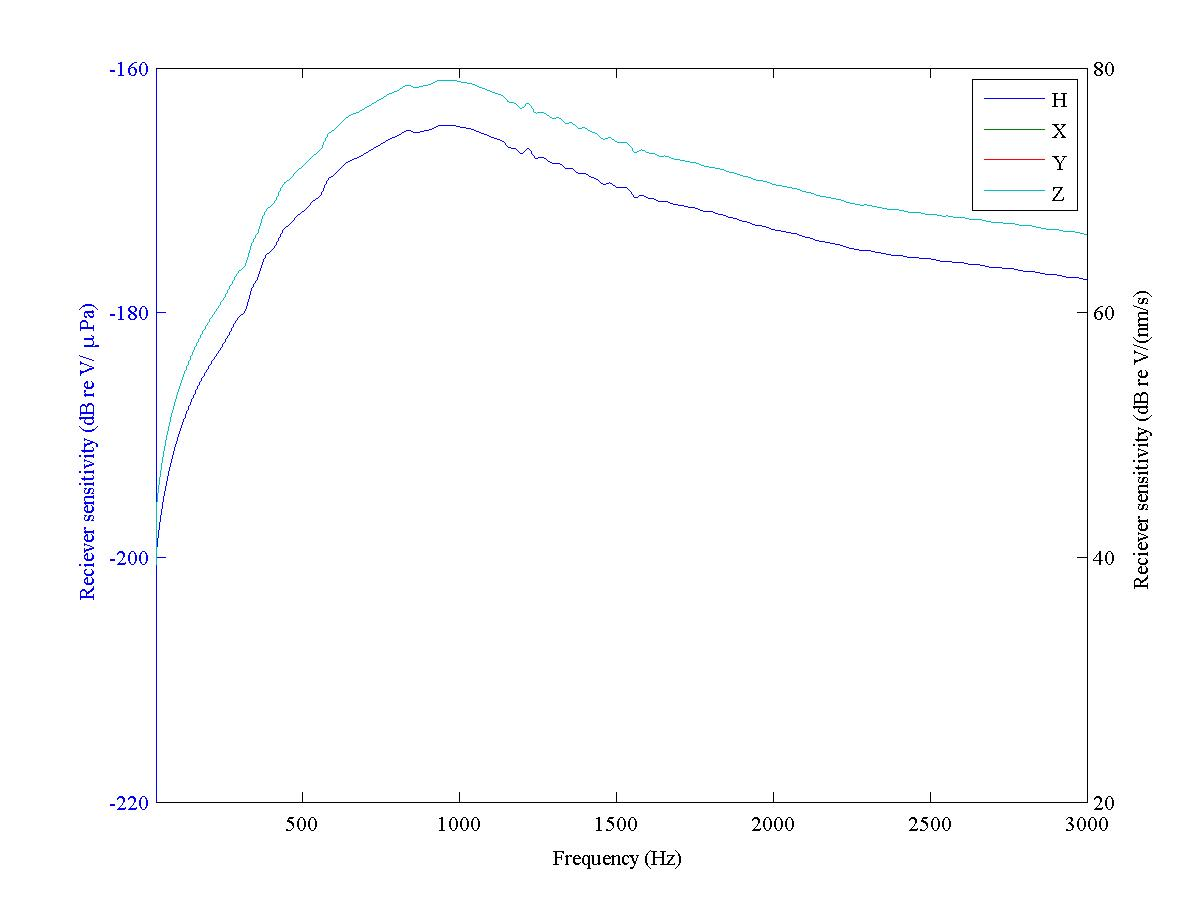
\includegraphics[width = \textwidth ]{12.jpeg}
\end{center}

\section{User Interface}

The functionality of paPAM is based around a central graphical user interface (GUI) which houses all the options you need to conduct your analysis.  Below is a brief summary of what the different sections of the GUI are used for:\\

\begin{center}
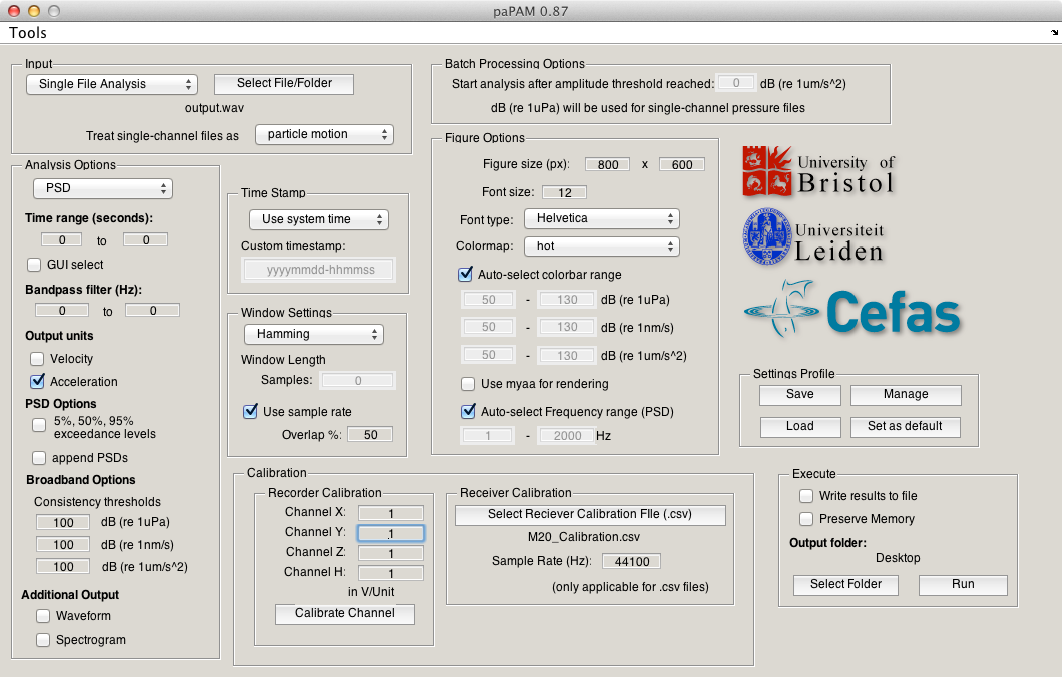
\includegraphics[width = \textwidth ]{3.png}
\end{center}

\subsection{Input}
Here you can select which file or folder you'd like to analyze.  Input files can be in the following formats:

\begin{itemize}
\item \texttt{wav \& mp3}: Channels \texttt{[1 2 3 4]} in the audio file represent channels \texttt{[X Y Z Hydrophone]} of a vector sensor.

\item \texttt{csv}: Columns \texttt{[1 2 3 4]} represent the \texttt{[x y z hydrophone]} channels, respectively.  If the columns have different lengths, the file will be truncated to the shortest column length to make sure there are an equal number of samples in each channel.
\end{itemize}

Each file type can hold up to 4 channels, so the x, y, z, and hydrophone data can all be stored in a single file for a given recording session.  If your data is currently stored as single channel wav files, see section \ref{CreatingMultiChannelWavFiles} for instructions on how to convert them to multi-channel wav files for easier storage and processing, or you can use the freely available program \texttt{Audacity} to make multi-channel audio files.

\subsubsection{Calibration Options}
The \texttt{Select Receiver Calibration File} selector is where you specify the location of the receiver calibration file (see \ref{CalibrationFiles}). For \texttt{wav} and \texttt{mp3} files, the sample rate will be extracted from the file automatically by paPAM. For csv files, you'll have to manually specify the sample rate you used during data logging in the \texttt{Sample Rate (Hz)} field.

\subsubsection{Single channel files}
For processing single channel wav files, you can specify if the first (and only) channel is either particle motion data or pressure data via the option \texttt{Treat single-channel files as}.

\subsubsection{Single or Batch Analysis}

For situations where you want to run the exact same analysis on multiple
files, you can specify a \texttt{Batch analysis}. paPAM will analyze all files located
in the specified folder, as opposed to a \texttt{single file analysis} where only
the specified file will be analyzed. When executing a \texttt{batch analysis}, all the
options you define for the first file for analysis will be repeated
on each proceeding file. More information about batch processing can be
seen in section \ref{BatchProcessingOptions}.

\subsubsection{Subsampling large files}
While the default MATLAB commands for reading audio or \texttt{csv} files are restricted by the amount of memory on your computer, paPAM employs modified versions of these respective importing functions so that your raw data is stored on your harddrive instead of memory.  This means that paPAM bypasses the typical size restrictions in file imports, as you are restricted by the amount of free space on your hard drive instead.  While you can select files of extremely large sizes, the regions you define within those files for analysis are still restricted by your RAM.

This feature is particularly useful if you want to analyze many small subsections of a large recording which cannot fit into memory.  Instead of cutting the audio file into multiple, smaller files, you can load the entire file into paPAM, then add an extra analysis for each subsection of the recording you want to analyze.

For example:  On a computer with 2GB of free memory, paPAM will allow you to select \texttt{wav} files of up to 4GB (the size limitation of the \texttt{wav} file format).  However, when selecting the time range for each analysis sample  within that file, these time ranges must select portions of the file which are less than 2GB in size.  This feature allows you to skip the step typically required by MATLAB analysis where you have to trim your large wav file in an external program before reading it with MATLAB.

\subsection{Recorder Calibration}

In the event that your recorder adds or reduces the gain on your vector sensor during data logging, you can correct for this effect by using the \texttt{Channel} fields in the \texttt{recorder calibration} section.  As an example, for a gain of \texttt{10dB} applied to your vector sensor measurements during logging (which you might do to increase the resolution of your data and reduce the effects of electrical noise), you would enter a value of \texttt{3.16} in the appropriate \texttt{channel} field. $$1\cdot10^\frac{10dB}{20} = 3.16\  \mathit{V/unit}$$

paPAM can also automatically calculate the recorder calibration ratios (i.e. recorder gain) from recorded pure tones with the following steps:
\begin{enumerate}
\item Record a sine wave (pure tone) of a known voltage directly into your recorder (i.e without the sensor) at the same recording level you used during data collection. For this you'll need an oscilloscope to measure the voltage.

\begin{itemize}
\item You can create a pure tone playback file within paPAM under \texttt{Tools > Create Calibration Tone}.
\end{itemize}

\item Then in paPAM, click \texttt{calibrate channel} in the \texttt{Recorder Calibration} section, enter your known peak-to-peak voltage (\texttt{Reference Voltage}) which you previously measured with your oscilloscope (vpp, in Volts), and select the channel you wish to calibrate.

\item Finally, you can graphically select the start and end points of the calibration file.  The maximum peak-to-peak voltage will be calculated from within this region.  After selection, the \texttt{Recorder Calibration} field for your selected channel will be automatically updated to the calculated calibration value.
\end{enumerate}

\subsection{Analysis Options}
The analysis options is where you can specify what types of analyses you will be using, in addition to the frequency time ranges for each analysis.

\subsubsection{Define an analyses type}
After selecting a file for analysis, you need to specify what type of analysis you'd like to conduct.  Three analysis types are included, each calculating a variety of metrics which are commonly used in underwater acoustic analyses.  For information on what metrics are calculated for each type, and how they are calculated, see section \ref{AnalysisTypes}.

\subsubsection{Define an analyses section}
After selecting an analysis type, if you would like to analyze a subsection of a file, as opposed to the whole file, this can be specified here (the default is that the full length and all calibrated frequencies will be analyzed).

\begin{itemize}
\item \textbf{Time range (seconds):}  The selected analysis type will be conducted between these start and end times.  If both fields are set to \texttt{0}, the entire file will be analyzed.
\item \textbf{Bandpass filter (Hz):}  A bandpass filter between this range will be applied to the section before analysis.  See section \ref{BandpassFilters} for more information about how bandpass filters are applied in paPAM.
\end{itemize}

For any given file, multiple analysis types can be run over multiple analysis sections in a single execution.  For more information on how to add multiple analysis types and sections to a file, see section \ref{Execute}.

\subsubsection{Output units}

The results and figures of your analysis will be displayed in the following units:
\begin{itemize}
\item \textbf{pressure} $(\mathit{dB\ re\ 1 \  \mu Pa})$
\item \textbf{velocity} $(\mathit{dB\ re\ 1 \ nm/s})$
\item \textbf{acceleration} $(\mathit{dB\ re\ 1\ \mu m/s^2})$
\end{itemize}

For particle motion channels, you can specify if the output is displayed in either velocity, acceleration, or both using the \texttt{Velocity} and \texttt{Acceleration} check boxes.

\subsubsection{PSD Options}
The options listed in this section are only applicable to power spectral density (PSD) analysis.  Checking \texttt{5\%, 50\%, 95\% exceedance levels} will output these metrics to both your figures and results file.  This is a useful metric for examining the variability over time of your analysis sample.

The append PSDs option is only recommended if you are encountering \texttt{Out of memory} errors during your analysis.  See \ref{MemoryIssues} for more information on how to use this option.

For more information regarding the different analysis options and how they are computed, see section \ref{AnalysisTypes}.

\subsubsection{Broadband Options}
Here you can specify the amplitude thresholds for pressure, velocity, and acceleration during broadband analysis.  These thresholds will be used in the consistency analysis (i.e. the percent of time that the amplitude is beyond the given threshold).

For more information regarding the different analysis options and how they are computed, see section \ref{AnalysisTypes}.

\subsubsection{Additional Output}
You can select some additional figures for output which are useful for proofing or publishing:
\begin{itemize}
	\item  \textbf{Waveform}\\
		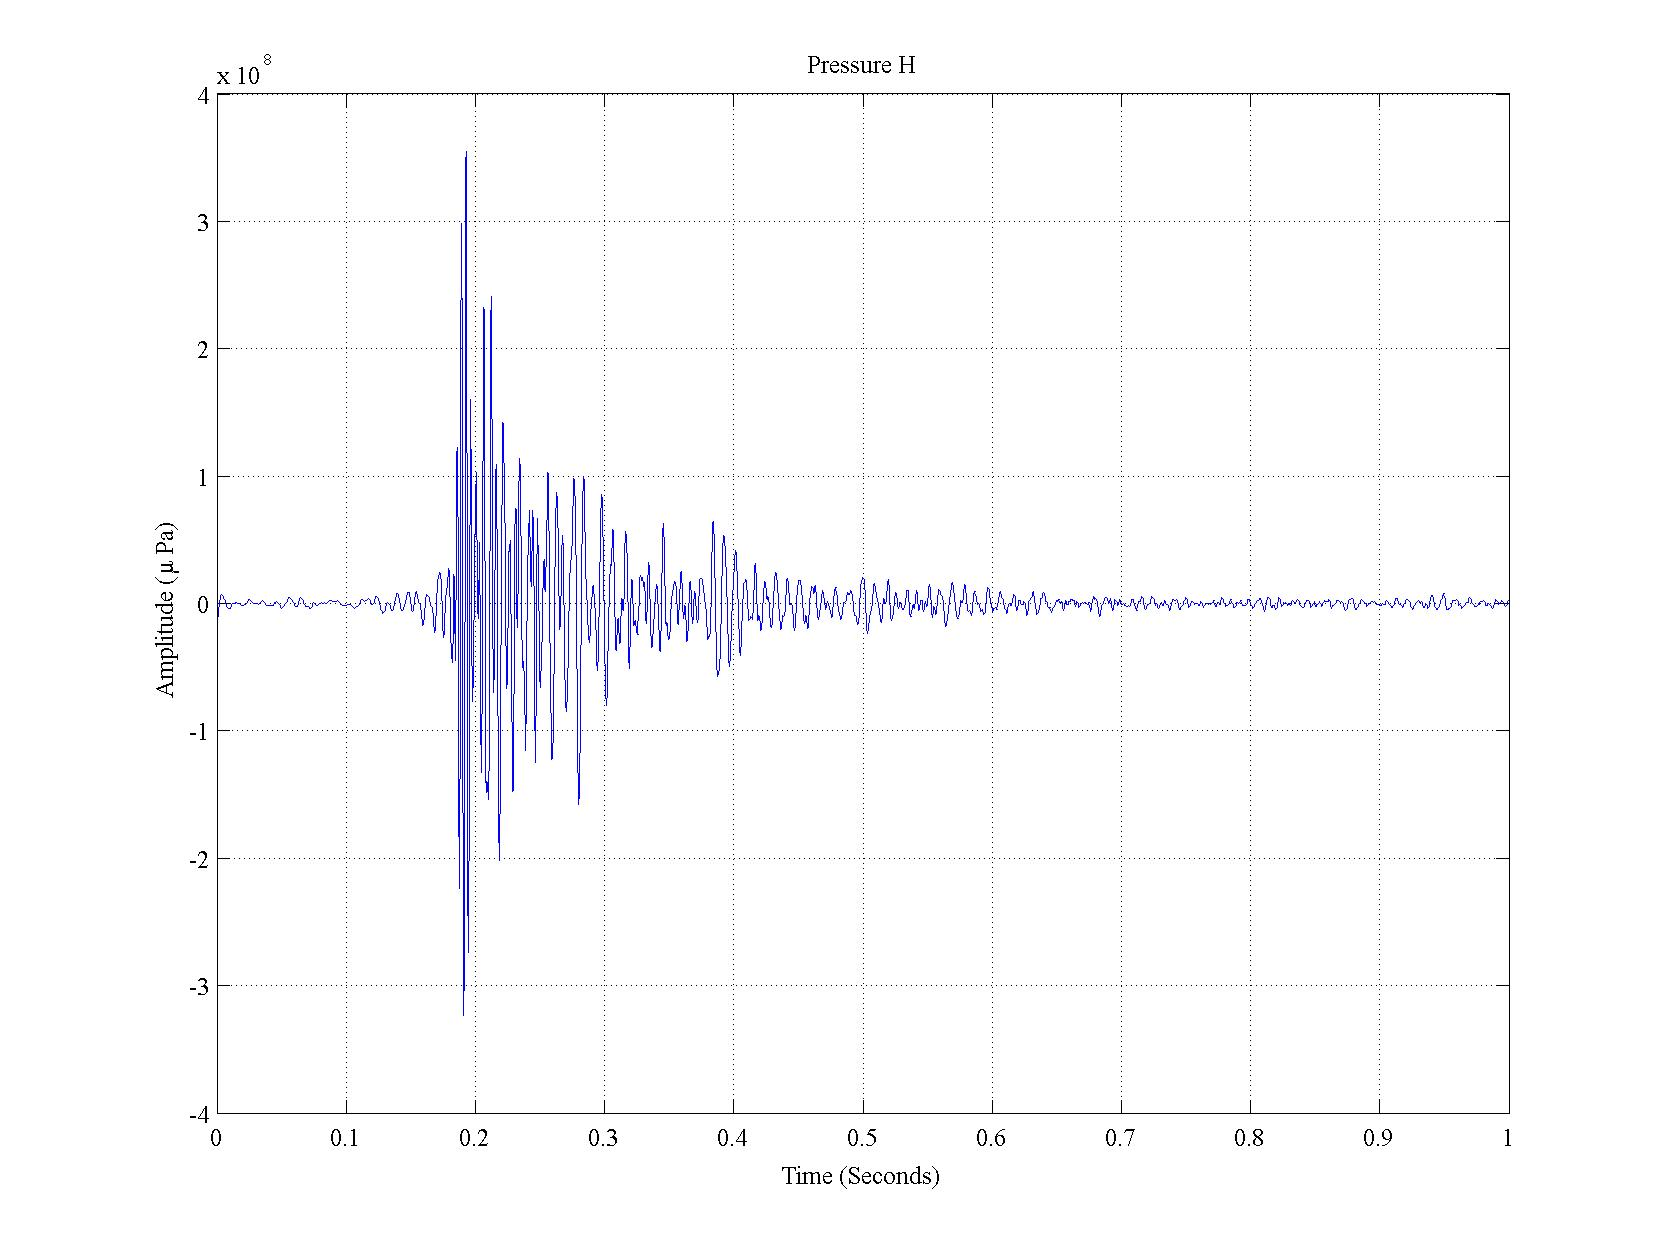
\includegraphics[width = \textwidth ]{11.jpeg}
	\item  \textbf{Spectrogram}\\
		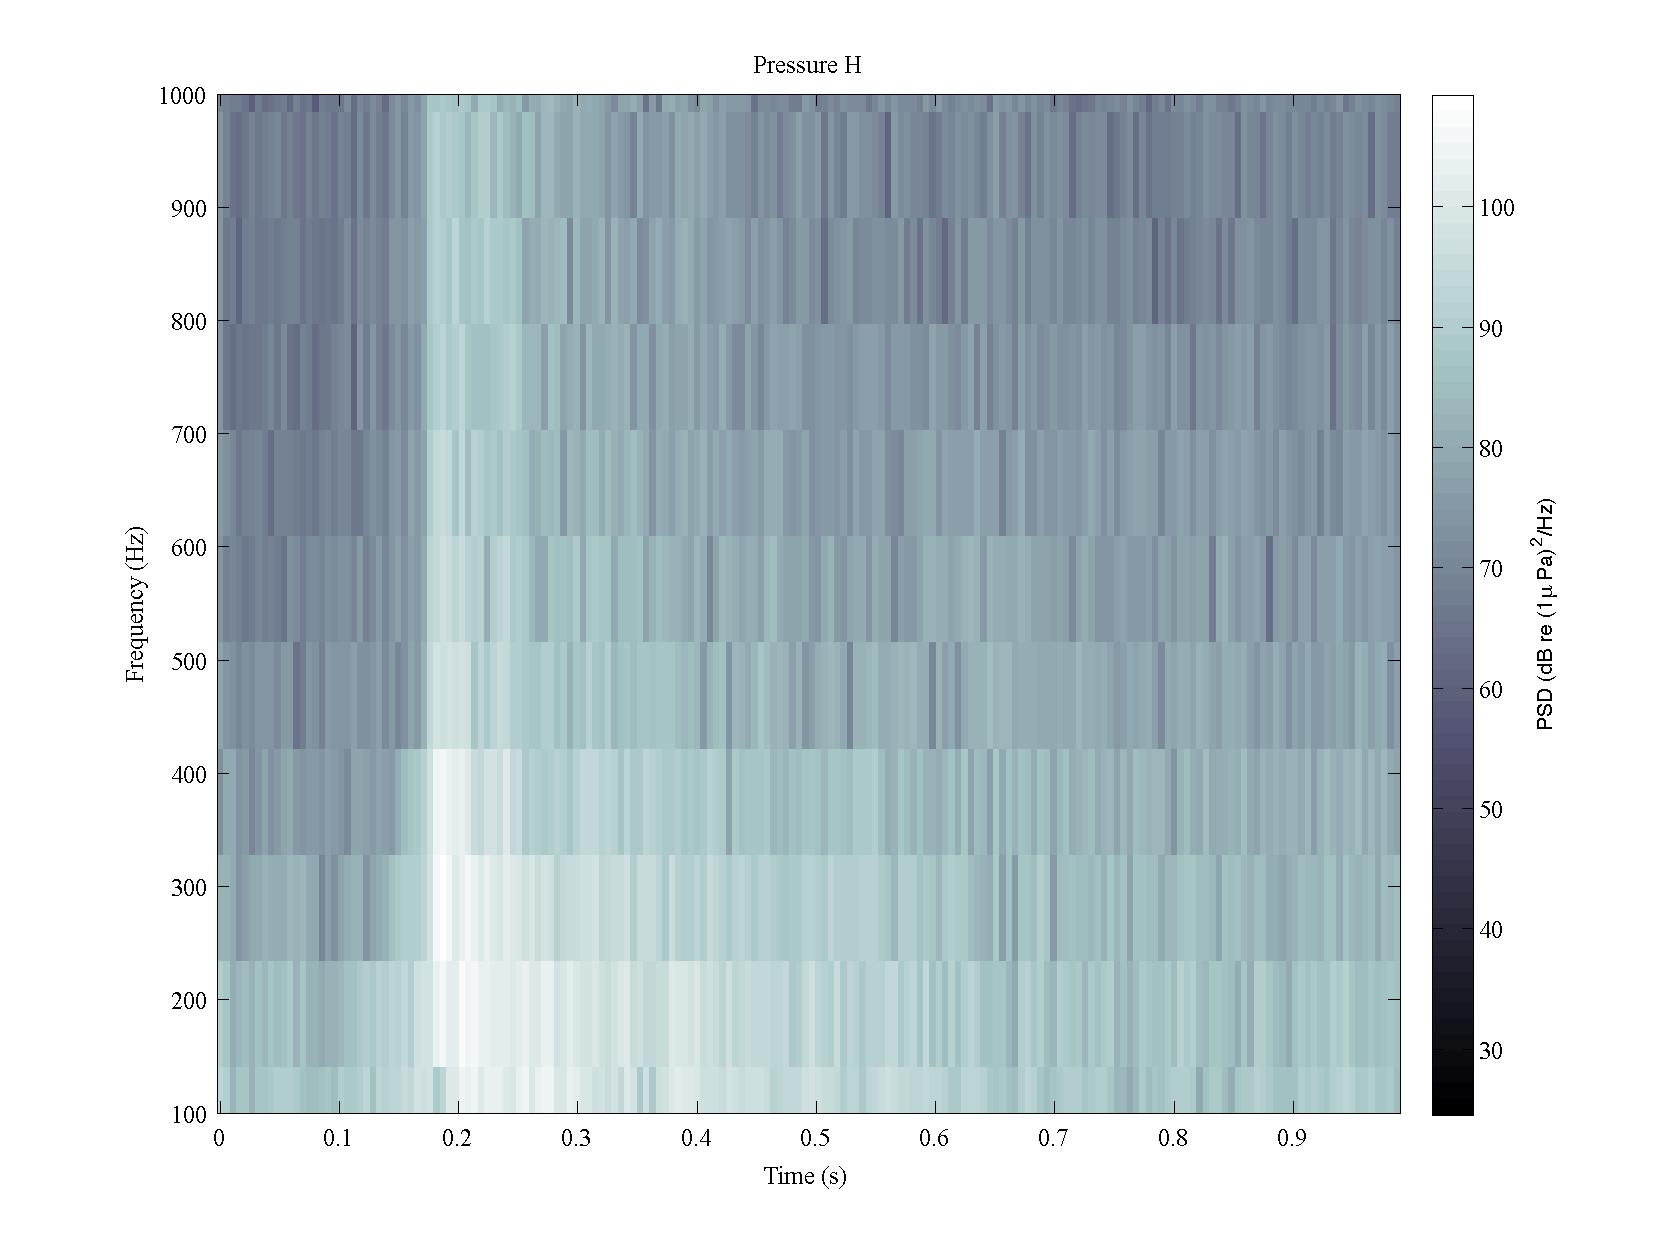
\includegraphics[width = \textwidth ]{10.jpeg}
\end{itemize}

You can adjust the appearance of these figures using the \texttt{Figure Options}.

\subsection{Window Settings}
\subsubsection{Window Length}
To compute a PSD, we divide the recording into sections of a defined length (\textit{windows}) before conducting a discrete Fourier transform (DFT) on each window. The number of samples in a window determines the temporal and frequency resolution of the analysis. By default, the \texttt{Window length} is set to your sampling frequency (Fs).  This results in a frequency resolution of 1 Hz and a temporal resolution of 1 s. Selecting a higher number than the Fs will give a lower temporal resolution and a higher frequency resolution, while numbers lower than the Fs will give a higher temporal resolution and a lower frequency resolution. Thus, the \texttt{Window Length} will affect the temporal and frequency resolution of your resulting PSD's.

In addition, your window length must be smaller than the total number of samples in your selected time range for the analysis. If you violate this restriction, a warning message will appear during your analysis.

\subsubsection{Window Type}
We apply a \textit{windowing filter} to each window to prevent \textit{spectral leakage} (an artifact of the computation process which reduces the accuracy of the resulting PSD).  A windowing filter attenuates the energy in the samples near the beginning and end of the window (this is often in the shape of a bell curve although there are many different types).   The windowing filter can be selected via the \texttt{Window type} selection box.  \textit{Hamming} is selected by default, but you may also select \textit{Hann} (Hamming and Hann windows are very similar and both are fine for PSDs).

\subsubsection{Overlap}

To compensate for the energy loss resulting from the \textit{windowing filter}, we allow windows to overlap.
By default, an overlap of 50\% is used. 50\% is sufficient to avoid losing energy due to windowing.  Overlapping by more than this will increase the amount of data produced and have the effect of \textit{smoothing} the spectrogram.

\subsection{Time Stamp}

When you begin your analysis, by default paPAM will note the current time on your computer and this will be printed in the names of all your resulting figures and results files.  All the files printed during a given execution of paPAM will share the same time stamp.  This allows you to match up the figures and results of each analysis execution for proofing.  If you want to set a custom time stamp (for example, if your system clock is not working correctly), you can specify a custom time stamp here.

\subsection{Batch Processing Options} \label{BatchProcessingOptions}
If you selected a specific time range for your analysis (as opposed to analyzing the entire file), the times selected for the beginning and end of each analysis sample in the first file will be carried over to all the remaining files during batch processing, thus it is important that all your files have synchronized starting points.  This is particularly important in impulse analyses, as a difference in a few milliseconds between your files may cause errors in the analysis.
To avoid the tedious task of manually clipping all your files, you can use the \texttt{Start analysis after amplitude threshold reached}.  Here's an example of how you'd use this feature:
\begin{enumerate}
\item If you are doing an impulse analysis with repeated strikes at constant intervals (10 seconds between strikes for example), you can use the occurrence of the first recorded strike to synchronize your files.
\item If the impulse sounds reach an amplitude of $130\ dB\ (re\ 1 \mu m/s)$ at your vector sensor, you can set your threshold value as $120\ dB\ (re\ 1 \mu m/s)$.  This will result in the beginning portion of the file, everything before the occurrence of the first strike, being removed from your analysis.
\item Now you can define your \texttt{time range} as \texttt{9.5-10.5} seconds.  All files will be synchronized so that 0 seconds in each file is set to the occurrence of the first impulse sound, and your impulse analysis will encompass the 1 second period when the next strike occurs.
\end{enumerate}

When using an oscilliscope to log your accelerometer data, it can often take some time before the logged voltage is normalized around zero once a recording has started.
The image below shows an example where the voltage started at an extreeme negative value on the start of logging, and gradually normalized after about a tenth of a second.
This behavior can cause triggering of your batch analsyis thresholds, before the desired point.
To circumvent this problem, you can set a value in the field \texttt{Skip first \_ seconds of file}.
Setting this to \texttt{1} will cause the thresold detection to start after skipping the first second of data, bypassing the region of the file which was not normalized around zero.

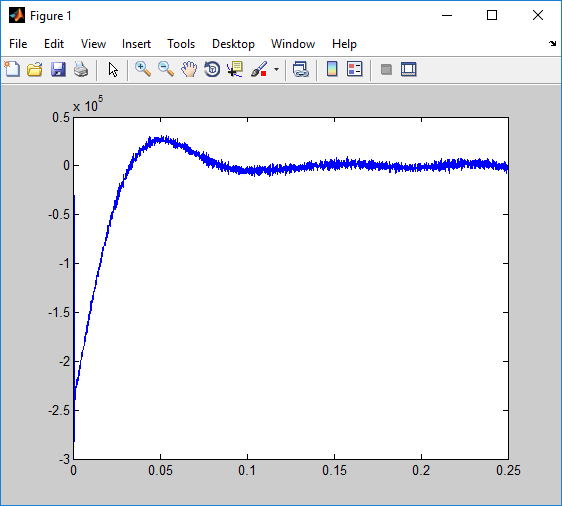
\includegraphics[scale=0.6,clip = true,trim = 0 0 0 0]{14.png}\\

\subsection{Settings Profile}
As it takes some time to configure all your analysis settings, you can save your current settings to a profile for quick access later on.  Press \texttt{Save} to save all your currently selected settings to a profile, and \texttt{Load} to load your previously saved settings.  By pressing \texttt{Set as default}, your current settings will be automatically loaded the next time you start paPAM.

\subsection{Execute} \label{Execute}

When you're ready to run your analysis, press \texttt{Select Folder} to set the location for your results and figures then press \texttt{Run} to start the analysis.  If \texttt{Write results to file} is not selected, you results will only be displayed in the MATLAB command window.

After the first analysis sample is processed (i.e. the first time range you defined), you will be asked if you want to process additional samples within the file:\\

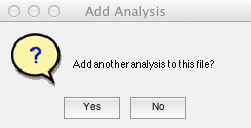
\includegraphics[scale=0.6,clip = true,trim = 0 0 0 0]{4.png}\\

If you select yes, the following window will open where you can define  additional samples to be analyzed:\\

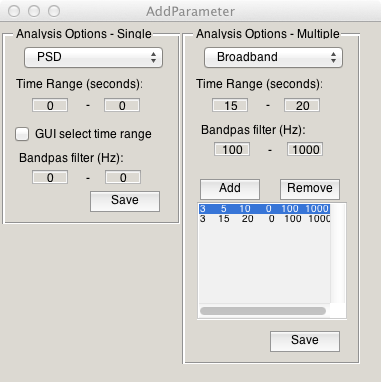
\includegraphics[scale=0.6,clip = true,trim = 0 0 0 0]{5.png}\\

To add a single additional sample, enter your parameters in the \texttt{Analysis Options - Single} and press \texttt{Save}.  In addition, you can add a series of additional samples to be analyzed in the \texttt{Analysis Options - Multiple} frame.  Use the \texttt{Add} and \texttt{Remove} buttons to populate the list box, and then press \texttt{Save} to execute the analyses.

When you analyze multiple samples within a file, the loading and calibration of the selected file will only occur once so the analyses will execute much faster as compared to defining all the samples and executing the analysis one-at-a-time from the main GUI.  For batch processing, all the samples you define in the first file will be analyzed on all the files found within the selected folder.

For information about the \texttt{Preserve Memory} option, see \ref{MemoryIssues}

\subsection{Figure Options}
Here you can define the appearance of your figures which are generated during analysis.

\subsubsection{Use myaa for rendering}
myaa is a freely available script downloaded from the Mathworks file exchange:

 \texttt{http://www.mathworks.com/matlabcentral/fileexchange/\\20979-myaa-my-anti-alias-for-matlab}\\

myaa was written by Anders Burn and can be used and distributed freely so long as the following copywrite notice is presented along with the use of myaa:

\begin{mdframed}[backgroundcolor = black!10]

Copyright (c) 2009, Anders Brun
All rights reserved.

Redistribution and use in source and binary forms, with or without
modification, are permitted provided that the following conditions are
met:

    * Redistributions of source code must retain the above copyright
      notice, this list of conditions and the following disclaimer.
    * Redistributions in binary form must reproduce the above copyright
      notice, this list of conditions and the following disclaimer in
      the documentation and/or other materials provided with the distribution

THIS SOFTWARE IS PROVIDED BY THE COPYRIGHT HOLDERS AND CONTRIBUTORS "AS IS"
AND ANY EXPRESS OR IMPLIED WARRANTIES, INCLUDING, BUT NOT LIMITED TO, THE
IMPLIED WARRANTIES OF MERCHANTABILITY AND FITNESS FOR A PARTICULAR PURPOSE
ARE DISCLAIMED. IN NO EVENT SHALL THE COPYRIGHT OWNER OR CONTRIBUTORS BE
LIABLE FOR ANY DIRECT, INDIRECT, INCIDENTAL, SPECIAL, EXEMPLARY, OR
CONSEQUENTIAL DAMAGES (INCLUDING, BUT NOT LIMITED TO, PROCUREMENT OF
SUBSTITUTE GOODS OR SERVICES; LOSS OF USE, DATA, OR PROFITS; OR BUSINESS
INTERRUPTION) HOWEVER CAUSED AND ON ANY THEORY OF LIABILITY, WHETHER IN
CONTRACT, STRICT LIABILITY, OR TORT (INCLUDING NEGLIGENCE OR OTHERWISE)
ARISING IN ANY WAY OUT OF THE USE OF THIS SOFTWARE, EVEN IF ADVISED OF THE
POSSIBILITY OF SUCH DAMAGE.

\end{mdframed}

Matlabs default renderer can produce saved images which look quite different from the figures they came from.  If you are having problems with the appearance of your saved images, you can try using \texttt{myaa} by selecting the \texttt{Use myaa for rendering}.  \texttt{myaa} does wysiwyg renderings and also applies its own anti-aliasing method to smooth out the resulting images.  This can be useful option if you are trying to make publishable, high quality figures.

Alternatively, if you want more control over the appearance of your figures, you can reopen the saved \texttt{.fig} files in matlab.  All the original data is stored within the \texttt{.fig} files, so you can rerender any figures you already saved through this method.

\subsection{Tools}

The \texttt{Tools} menu at the top of the GUI contains some additional features.

\subsubsection{Creating multi-channel \texttt{.wav} files} \label{CreatingMultiChannelWavFiles}


For easier storage and processing of your data, you can use the \texttt{Create multi-channel wav files} tool to convert single-channel wav files into multi-channel files.
If you have large amounts of data that you need to convert, you can use the \texttt{Batch} option to let paPAM scan a folder and automatically arrange \texttt{wav} files with similar names into multi-channel files.

To use the \texttt{Batch} feature, you need to specify the naming convention used by the \texttt{wav} files in the \texttt{Parsing mask} field.  In the \texttt{Batch} GUI, there are a variety of examples and instructions on how to enter a correct \texttt{Parsing mask}.

\section{Bandpass Filters} \label{BandpassFilters}

During any analysis, a bandpass filter is applied to your data up to two times:
\begin{enumerate}
\item \textbf{Calibration Range:}  While paPAM is converting your raw data into calibrated units, a band pass filter is applied around the minimum and maximum defined calibration ranges.  This is to ensure that any sounds occurring outside your calibrated range do not influence your analysis.
\item \textbf{Analysis Range:} In the \texttt{Analysis options}, the user can specify a bandpass range to be applied.  This bandpass filter is applied in addition to the bandpass filter already applied to the calibration range.  If the user selected $0 \ \mathtt{Hz}$ for their \texttt{low pass} range (maximum frequency), no bandpass will be used here.
\end{enumerate}
\begin{samepage}
All bandpass filters in paPAM are executed in the same manner.  Below is the matlab code used for each bandpass:

\begin{lstlisting}
% Define butter filter
[b,a] = butter(3,[HighPassFrequency LowPassFrequency]./...
	(SampleRate./2));
% Apply filter to selected data
output = filter(b,a,data);
\end{lstlisting}
\end{samepage}

\chapter{Analysis Types} \label{AnalysisTypes}

This section contains detailed information on how each metric is calculated in paPAM.  When applicable, both the an example of matlab code (gray boxes), and the mathematical formulas for each analysis are given.

\section{PSD}

\begin{center}
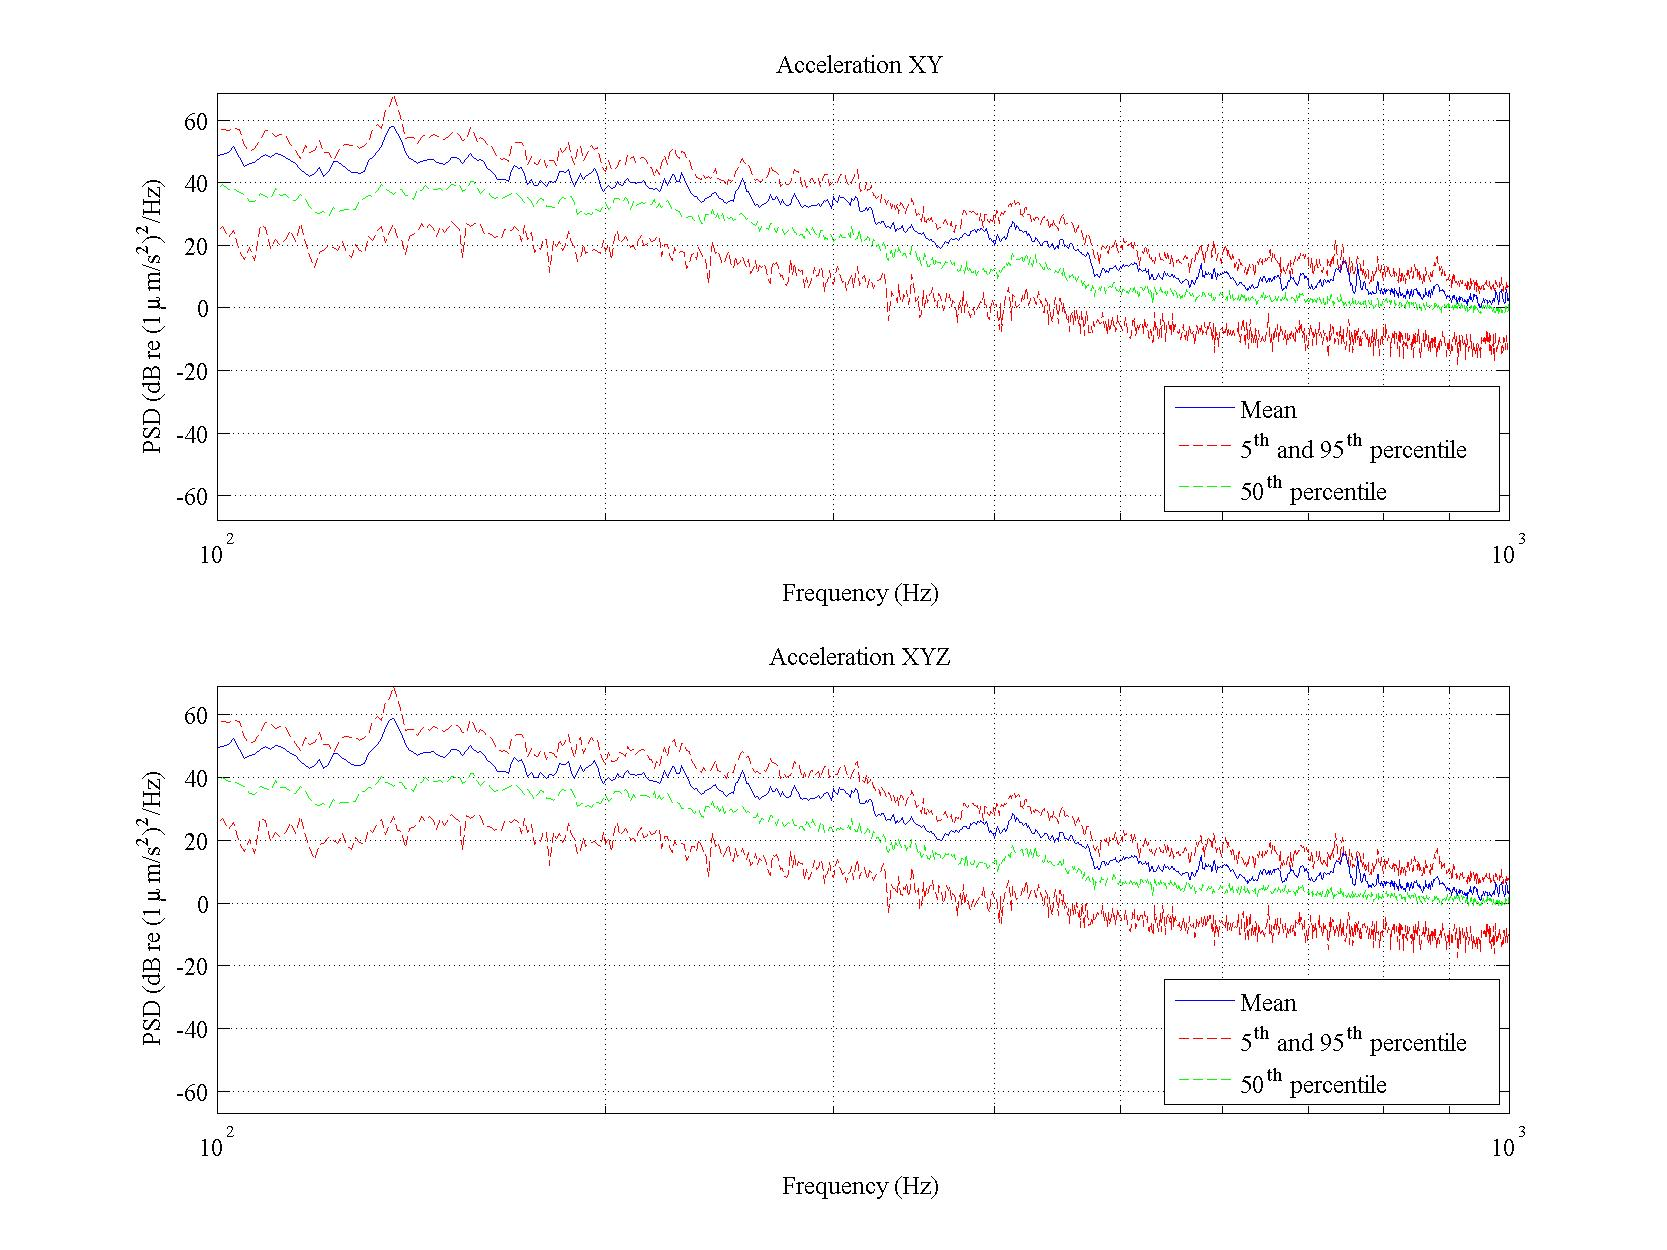
\includegraphics[width = \textwidth ]{7.jpeg}
\end{center}

The PSD analysis will produce PSD figures in addition to \texttt{csv} files reporting the dB power levels for each window segment in the analysis.  On the main GUI, the options which affect the PSD figures and results are:
\begin{itemize}
\item Window Settings
\begin{itemize}
\item Window type:\\
In this version of paPAM, only the Hamming window is active and will be selected automatically.  Other window types will be implemented in later versions of paPAM
\item Window length
\item Overlap
\end{itemize}
\item 5\%, 50\%, 95\% exceedance levels:\\
This option is useful for examining the variance between each window segment of the PSD.
\end{itemize}

The following MATLAB code is used to generate the PSD's:

\begin{lstlisting}
%Chop waveform into segments
data2ch1 = buffer(waveformData,nfft,ceil(nfft*olap*1e-2),...
'nodelay');
%olap = integer between 0 and 100

%% Define window type and constants
switch windowS{1}
	case 'Hann';
    	window = hann(windowL);
		windowScalingFactor = 0.54;
		noisePowerBandwidth = 1.36;
	case 'Hamming';
		window = hamming(windowL);
		windowScalingFactor = 0.5;
		noisePowerBandwidth = 1.5;
end

%% FFT
%Apply scaling factor
[~,n] = size(data2ch1);
data2ch1 = data2ch1.*repmat(window,1,n)/windowScalingFactor;
%fft
fft_data_ch1 = abs(fft(data2ch1))./nfft;
fft_amp_ch1=fft_data_ch1(1:nfft/2+1,:).^2;
% Correction for the noise power bandwidwith
fft_amp_ch1=2*fft_amp_ch1/noisePowerBandwidth;
% Deriving the frequency units
f = (Fs/2*linspace(0,1,nfft/2+1))';
% Normalizing for 1 second
wintime = nfft/Fs;      %time in seconds of window
acc1 = fft_amp_ch1*wintime;

%%  Calculate results
% Mean
Xmean = mean(acc1,2);
% Percentiles
X5 = prctile(acc1,5,2);
Xmedian = prctile(acc1,50,2);
X95 = prctile(acc1,95,2);
\end{lstlisting}

For PSD's calculated across multiple channels, the resulting power values calculated form the above function for each channel per frequency are summed using vector addition: \\

$$PSD(f)_{xyz} = \sqrt{PSD(f)_x^2 + PSD(f)_y^2 + PSD(f)_z^2}$$

\begin{flushright}
$f = \mathtt{Frequency}$
\end{flushright}

\begin{lstlisting}
%PSD's are vectors containing the calculated
%power values for each frequency in F
PSDxyz = sqrt(PSDx.^2 + PSDy.^2 + PSDz.^2);
plot(F,PSDxyz) % plot resulting PSD;
\end{lstlisting}

\section{Impulse}

\begin{center}
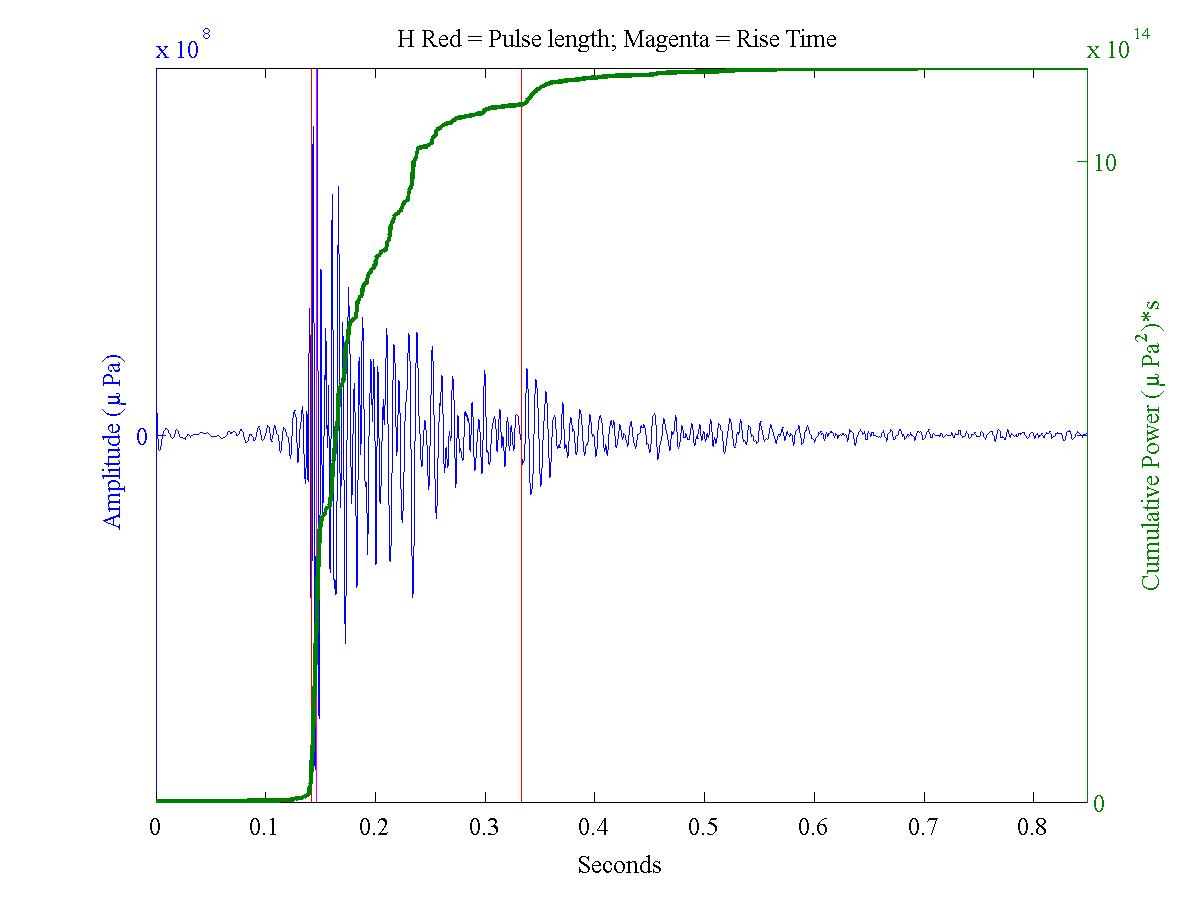
\includegraphics[width = \textwidth ]{8.jpeg}
\end{center}

The impulse analysis gives the following outputs, each of which can be calculated for pressure, velocity, and acceleration:\\
\begin{itemize}
\item \textbf{Zero-to-peak}
$$\mathit{max}|\mathit{p(t)}|$$
\begin{flushright}
$t = \mathtt{time}$
\end{flushright}

\begin{lstlisting}
zeroToPeak = max(abs(p));
%where p is a vector containing all the calibrated
%pressure values over time (uPa)

%For multiple channels combined
zeroToPeakxyz = max(sqrt(x.^2 + y.^2 + z.^2));

% where x, y and z are vectors containing the calibrated
% particle motion waveforms for each channel
% (units are in either nm/s or um/s^2)

\end{lstlisting}


\item \textbf{90\% energy envelope}\\\\
This represents the time interval between the first occurrence of the $5^{th}$ and $95^{th}$ cumulative energy percentile in the analysis region, where the cumulative energy at any given point in time, $t_n$, is defined by:\\
$$\sum_{t = 1}^{n}p(t)^2 dt$$
\begin{flushright}
$p$ = pressure
\end{flushright}

\begin{lstlisting}
dt = 1/sampleRate;
cumulativeEnergy = sum(p.^2)*dt;
\end{lstlisting}


For velocity and acceleration, pressure, $p$, is replaced by either $u$ or $a$.  When calculating the energy envelope across multiple particle motion channels, the following approach is used:\\

$$\sum_{t_ = 1}^{n} \left( u(t)_x^2 + u(t)_y^2 + u(t)_z^2 \right) dt$$

\begin{lstlisting}
cumulativeEnergy = sum(x.^2 + y.^2 + z.^2)*dt;
\end{lstlisting}

\item \textbf{Single-strike exposure}

The single-strike exposure is defined as the sound exposure within the period encompassing the 90\% energy envelope.  Exposure is calculated in the same way as cumulative energy:\\

$$ \sum_{t = 1}^{n}p(t)^2 dt $$

\item \textbf{Crest factor}

Crest factor is defined as the zero-to-peak sound pressure divided by the root-mean-squared sound pressure:\\

$$ \frac{\mathit{max}|\mathit{p(t)}|}{\sqrt{\frac{1}{n} \sum_{t = 1}^{n}p(t)^2}} $$

\begin{lstlisting}
crestFactor = max(p)/(rms(p));
\end{lstlisting}

For particle motion calculated over multiple channels, the crest factor is defined as:

$$ \frac{\mathit{max}\left( \sqrt{u(t)_x^2 + u(t)_y^2 + u(t)_z^2} \right)}{\sqrt{\left(\frac{1}{n} \sum_{t = 1}^{n}u(t)^2_x \right) + \left(\frac{1}{n} \sum_{t = 1}^{n}u(t)^2_y \right) + \left(\frac{1}{n} \sum_{t = 1}^{n}u(t)^2_z \right)}} $$

\begin{lstlisting}
crestFactorXYZ = max(sqrt(x.^2 + y.^2 + z.^2))/...
sqrt(rms(x).^2 + rms(y).^2 +  rms(z).^2);
\end{lstlisting}

\end{itemize}
\section{Broadband}

This analysis calculates the following metrics for pressure, velocity, and acceleration:

\begin{itemize}
\item \textbf{Root-mean-square pressure/particle motion}

This is the root-mean-squared sound pressure over the specified time range.

$$ \sqrt{\frac{1}{n} \sum_{t  =1}^{n}p(t)^2} $$

\begin{lstlisting}
rms(p);
\end{lstlisting}

For measurements combined over multiple particle motion channels, the root-mean-square velocity or acceleration is calculated separately for each channel, then combined according to vector addition:

$$\sqrt{\left(\frac{1}{n} \sum_{t = 1}^{n}u(t)^2_x \right) + \left(\frac{1}{n} \sum_{t = 1}^{n}u(t)_y^2 \right) + \left(\frac{1}{n} \sum_{t = 1}^{n}u(t)^2_z \right)}$$

\begin{lstlisting}
sqrt(rms(x).^2 + rms(y).^2 + rms(z).^2);
\end{lstlisting}

\item \textbf{Sound Exposure}

Sound exposure is calculated over the specified time range:

$$ \sum_{t = 1}^{n}p(t)^2 dt $$

\begin{lstlisting}
dt = 1/sampleRate;
SoundExposure = sum(p.^2)*dt;
\end{lstlisting}

As with the root-mean-squared metric, the results for combined particle motion channels are summed together with vector addition:

$$ \sqrt{\left(\sum_{t = 1}^{n}u(t)_x^2 dt \right)^2 + \left(\sum_{t = 1}^{n}u(t)^2_y dt \right)^2 + \left( \sum_{t = 1}^{n}u(t)^2_z dt \right)^2 }$$

\begin{lstlisting}
SoundExposureXYZ = sqrt((sum(x.^2)*dt).^2 +...
 (sum(y.^2)*dt).^2 + (sum(z.^2)*dt).^2) ;
\end{lstlisting}

\item \textbf{Consistency Analysis}

The consistency analysis calculates the percent of the time in which the amplitude of the signal exceeds a user defined threshold.  The following code describes how consistency is calculated over a single channel:

\begin{lstlisting}
% data = waveform data

%Count number of times the
% threshold was exceeded in waveform
countExceedThreshold =...
 sum(data < -1*(10^(dBthreshold/20))) ...
+ sum(data > (10^(dBthreshold/20)))
% Convert to percentage
consistency = countExceedThreshold*100/...
length(data)
\end{lstlisting}

and for multiple channels:
\begin{lstlisting}
% dataX = X channel waveform data
% dataY = Y channel waveform data
% dataZ = Z channel waveform data

data = sqrt(dataX^2 + dataY^2 + dataZ^2)

%Count number of times the threshold
% was exceeded in waveform
countExceedThreshold =...
 sum(data < -1*(10^(dBthreshold/20))) ...
+ sum(data > (10^(dBthreshold/20)))
% Convert to percentage
consistency = countExceedThreshold*100/...
length(data)
\end{lstlisting}

\end{itemize}

\chapter{Advanced features}
\section{Memory Issues} \label{MemoryIssues}

While paPAM saves all your calibrated data to the hard drive, MATLAB requires free RAM to execute the functions which are used in each analysis.  On computers with low amounts of memory, an \texttt{Out of memory} error may occur when analyzing large segments of data.  To workaround and avoid these errors, you can try the following steps.

\begin{enumerate}
\item \textbf{Preserve Memory}.
By selecting the \texttt{Preserve Memory} option from the \texttt{Execute} section on the main GUI, you can free up large portions of RAM during your analyses. Figures in MATLAB take up considerable amounts of memory, so having multiple figures open at once during the analysis can severely restrict the memory available.  By checking the \texttt{Preserve Memory} option, paPAM will close each figure after it has been  generated and saved to your hard disk, thus freeing up memory for your analysis.  This can be especially useful when you want to save Spectrogram images during your analysis, as Spectrogram figures can easily take up over 100MB per figure.

\item \textbf{append PSDs}.
This option is useful if you want to conduct a PSD analysis over a large region, but paPAM keeps on hitting an
\texttt{Out of memory} error.  As a workaround, you can divide your PSD analysis into several smaller PSD analyses.  When you check the \texttt{append PSDs} option, paPAM will combine the window segments generated from each PSD analysis into a single PSD result where the percentiles can be calculated.  For example:

\begin{enumerate}

\item Suppose you want to construct a PSD which spans from 0-500 seconds in your \texttt{example.wav} file, but when you try to execute the analysis, you recieve an \texttt{Out of memory} error.

\item To workaround this limitation, you check the option \texttt{append PSDs} on the main GUI, and select the time range 0-100 seconds for your first PSD analysis.

\item After the analysis has completed, you will be asked \texttt{Would you like to add another analysis to this file?}  Select \texttt{Yes}, and in the \texttt{Analysis Options - Multiple} section, add 4 more PSD analyses which span the ranges 100-200, 200-300, 300-400, and 400-500 seconds.  Press \texttt{save} and allow the analysis to run to completion.  The file \texttt{appendedPSD.csv} in your results folder will now contain the results of a PSD analysis which was conducted over the window segments of all 5 PSD analysis you did combined.

\end{enumerate}

Here is some example output from the \texttt{append PSDs} feature:

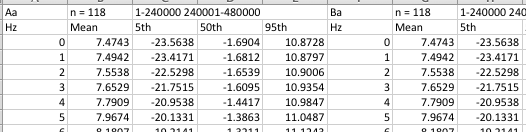
\includegraphics[scale=0.6,clip = true,trim = 0 0 0 0]{6.png}\\

\begin{itemize}
\item The cell \texttt{A1} holds the name of the channel analyzed, where $[A\ B\ C\ D]$ represent the $[X\ Y\ Z\ Hydrophone]$ channels.  Channel calculated for acceleration are represented with a proceeding lowercase $a$, $[Xa\ Ya\ Za]$ , while velocity channels have no proceeding $a$, $[X\ Y\ Z]$.

\item The cell \texttt{B1} denotes the number of window segments used in the calculation.  This is useful as an error checking tool.

\item The cell \texttt{C1} holds information about the sample ranges included in each analysis by showing the start and end samples of each PSD included in the analysis.  A range of \texttt{1-240000 240001-480000} tells that 2 PSD analysis were used in the calculation, and each PSD analysis contained 240000 samples and there is no gap in between the PSD segments.
\end{itemize}

\end{enumerate}

\chapter{paPAM Calculator}

\section{Intro and Setup}
paPAM calculator is a tool you can use to predict the particle velocity and acceleration derived from measured pressure values.  By comparing your predicted particle motion values to your measured particle motion values, paPAM calculator can be used as a rough proofing tool to check for major errors in your receiver calibration.

Setting up the paPAM Calculator requires the exact same steps found in section \ref{SettingUppaPAM}.  For full versions of MATLAB, you'll want to run the file in the \texttt{paPAM\_Calculator} folder:

\begin{itemize}
\item \texttt{PM\_Analysis\_Modeling.m}
\end{itemize}

To run paPAM using MCR, you'll use the following files:

\begin{itemize}
\item Mac
\begin{itemize}
\item \texttt{paPAM\_Calculator\_mac.app}
\item \texttt{run\_paPAM\_Calculator\_mac.sh}
\end{itemize}
\item Windows
\begin{itemize}
\item \texttt{paPAM\_Calculator\_win.exe}
\end{itemize}
\end{itemize}


\section{Interface}
Like paPAM, the paPAM calculator is built upon a central GUI:

\begin{center}
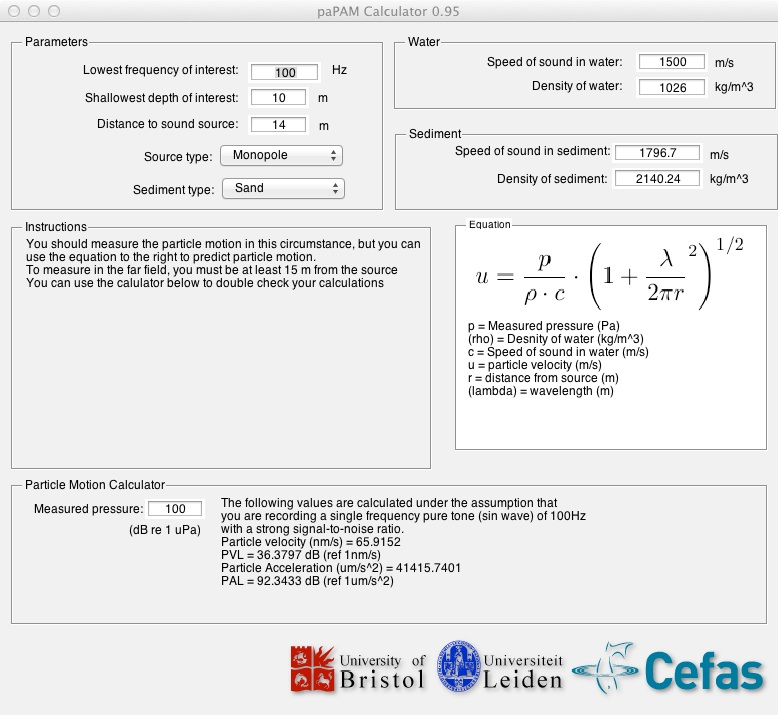
\includegraphics[width = \textwidth ]{13.jpg}
\end{center}

As you enter values into the text boxes, the calculator will automatically update and provide measurement recommendations based on your parameters.  In the fields \texttt{Lowest frequency of interest} and \texttt{Shallowest depth of interest}, the lowest frequency is the lowest frequency you are interested in analyzing and the shallowest depth refers to the shallowest depth along the direct path between the sound source and the hydrophone.

After you have selected your parameters, you can enter in a \textit{dB} value in the \texttt{Particle Motion Calculator} to estimate the particle motion values.  Because some of the equations used to predict particle motion are dependent on frequency, all velocity and acceleration numbers presented are assuming that you are measuring a single pure tone sound which has a frequency defined by the \texttt{Lowest frequency of interest} you selected.

\section{Equations}
The paPAM calculator employs 3 commonly used acoustic equations to predict particle motion.  These equations are listed below:

\begin{itemize}
\item Near-field particle velocity from pressure:
$$u = \frac{p}{\rho \cdot c} \cdot \left(1 + \frac{\lambda}{2 \pi r}^2 \right)^{1/2}$$
\begin{flushleft}
$u$ = particle velocity ($m/s$)\\
$p$ = acoustic pressure($m/s$)\\
$\rho$ = density of water ($kg/m^3$)\\
$\lambda $ = wavelength of frequency of interest ($m$)\\
$r$ = distance from source ($m$)\\
$c$ = speed of sound in water ($m/s$)\\
\end{flushleft}
\item Far-field particle velocity from pressure:
$$u = \frac{p}{\rho \cdot c}$$
\item Cut-off frequency (for open-water environments):
$$f_c = \frac{\pi - \rho_{sed}/\rho_{water}}{2 \cdot \pi \cdot \sin \left( \arccos \left( c/c_{sed} \right) \right)} \cdot \frac{c}{H}$$
\begin{flushleft}
$\rho_{sed}$ = density of sediment ($kg/m^3$)\\
$\rho_{wat}$ = density of water ($kg/m^3$)\\
$c_{sed}$ = speed of sound in sediment ($m/s$)\\
$H$ = Depth of water ($m$)\\
\end{flushleft}
\end{itemize}

\end{document}
